\documentclass{article}
\usepackage{graphicx}

\author{John Hammond}
\title{TE 401 Final Presentation FA19}

\begin{document}

%title followed by blank space before next pager
\maketitle
\tableofcontents
\newpage

%introduction and background on the project
\section{Motivation for the Augmented Listening Project}
Augmented listening and the work we are doing here will change the way we hear and perceive\
the world around us. The idea of augmented listening is to utilize microphone arrays of any size to alter the way we hear audio.\
Effects such as source separation, dynamic range compression, and selective attenuation are all examples of digital signal\
processing in the context of hearing. Devices like hearing aids are very common and help people by amplifying the sounds around\
them and performing basic dynamic range compression.  Hearing aids, however, are limited in their capabilities due to the small\
number of microphones available and the relatively small amount of processing power. They struggle in loud environments\
with multiple sources as well as reverberant environments.  Hearing aids are only one example of augmented listening\
technology, and applications go far beyond this.

We aim to create\
an open hardware platform with support for large numbers of microphones and complex signal processing algorithms.\
This hardware platform will function as a proof of concept for our own signal processing applications as well as those\
of other researchers across the world.  The basic platform is based upon a Cyclone\textsuperscript{\textregistered{}}\
V SoC system, with support for both\
hardware logic and software applications on the ARM cores. Our implementation supports I2S microphone data streams as\
inputs for processing.

%descripton of current hardware
\section{Current Hardware Platform}

\subsection{FPGA}
The FPGA is programmed to receive I2S data, store samples in DDR3 memory buffers, and to support real-time\
signal processing cores.  We will mostly describe the hardware as it relates to recording.

\subsubsection{I2S}
Our array prototypes have all consisted of MEMS mcirophones, which send their bitstream over the I2S bus.\
We chose these microphones because they are very cheap and easy to prototype with. Two microphones share a sample\
clock, right/left select clock, power, and a data line. The right and left channel alternate sending thier 16\
bit samples. These samples are then pieced together at the I2S master into a coherent right and left data\
stream. These master cores are implemented in the FPGA fabric. Refer to figure\
\ref{i2s_timing} for an example of\
a typical I2S data transfer.

\begin{figure}[ht]
	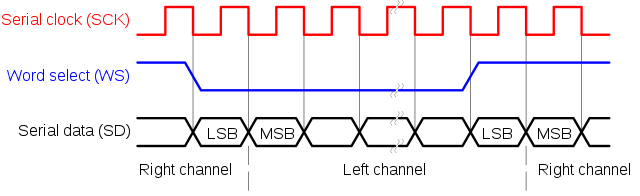
\includegraphics[scale=.5]{pictures/i2s_timing.png}
	\centering
	\caption{I2S timing diagram (wikipedia citation needed)}
	\label{i2s_timing}
\end{figure}

\newpage

\subsubsection{DMA Controller and Buffers}
Recording audio from a large number of microphones is a challenge and is one of the\
features of our\
open platform. There is 7.68 Mbit of space allocated in memory for the samples from\
each of the 10\
microphones. Each of the five I2S masters hold the latest valid 16-bit sample for each\
microphone on its output register. The DMA controller then iterates through these 10\
registers and writes their values to the proper memory address.  These data transfers\
are all done over the Avalon\textsuperscript{\textregistered{}} bus. \

Figure \ref{dma_sim} shows the activity on the\
Avalon\textsuperscript{\textregistered{}} bus while the DMA controller is running.\
The microphone sample data is asserted on the AM\_WRITEDATA line.  The address of each\
sample is asserted on the AM\_ADDR line.  The DMA controller cycles through these\
addresses while recording, as seen in the sequence of 0x1000024, 0x01753024,\
0x01EA6024, 0x025F9024, and 0x02D4C024. The write enable signal AM\_WRITE stays high\
for the duration of these transfers.

\begin{figure}[ht]
	\begin{center}
	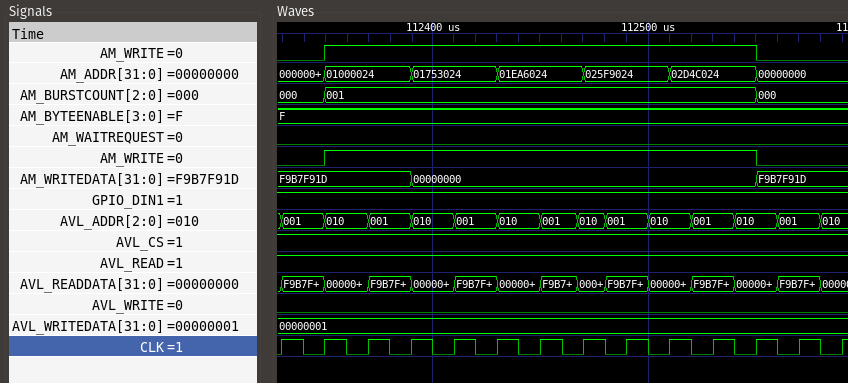
\includegraphics[scale=.4]{pictures/sim_close.png}
	\caption{Simulation of DMA access}
	\label{dma_sim}
	\end{center}
\end{figure}

\subsubsection{Filtering}
Real time signal processing can be performed in the FPGA fabric using hardware logic.\
Altera\textsuperscript{\textregistered{}} provides FIR filters as part of their\
university program.  

\subsection{HPS}

\subsubsection{Linux}
The hard processor system is based on two ARM Cortex-A9 cores.  On this processor we\ are running a lightweight GNU/Linux distribution to handle low level hardware control.\
File I/O, ftp, ssh, and ethernet controls are made very easy using the HPS as opposed\
to pure hardware logic. Altera\textsuperscript{\textregistered{}}'s provided OS image\
can be put on a microSD card and booted at power on.

\subsubsection{Recording and Processing}
On top of our Linux system we have a small C++ program to read samples from the DDR3\
buffer and store it or process it.  This is the second part of the recording process\
after the DDR3 buffers have been completely filled out by the DMA controller.\
This piece of code actually works similarly to the DMA in hardware just in\
reverse. Altera\textsuperscript{\textregistered{}} provides libraries with their HPS\
development environment to make the HPS interface nicer with the FPGA fabric.\
Specifically, the current recording program uses the mmap function to map the\
FPGA memory mapped addresses to addresses in the GNU/Linux userspace. These\
addresses are dereferenced in the C++ program to access the FPGA's hardware\
registers. This is more complex than using a soft core such as a RISC-V core\
or a ZipCPU because the hard processor cannot be reconfigured for any different\
hardware configuration.

\end{document}